\begin{table}[htbp]\centering\small
\begin{tabular}{lrrr}
\toprule
Policy & Mean infected & Hidden person-days & Tests \\
\midrule
No testing & 48.6\% & 1564 & 0 \\
Random & 39.2\% & 1030 & 840 \\
Degree & 18.6\% & 415 & 840 \\
Recent-contact & 20.1\% & 383 & 840 \\
Adaptive & 15.8\% & 303 & 840 \\
\bottomrule
\end{tabular}
\caption{Real Haslemere contact graph, stochastic disease simulation (mean across 50 outbreak replicates). All policies use the same observed contact graph and budget; results are not observed clinical infections.}
\label{tab:haslemere}
\end{table}
At $B=20$, the replicate-paired adaptive-minus-random attack-rate contrast is -23.36 percentage points (Monte Carlo 95\% interval [-26.82, -19.91] percentage points).
At $B=20$, the replicate-paired adaptive-minus-contact attack-rate contrast is -4.30 percentage points (Monte Carlo 95\% interval [-6.20, -2.40] percentage points).
\begin{figure}[htbp]\centering
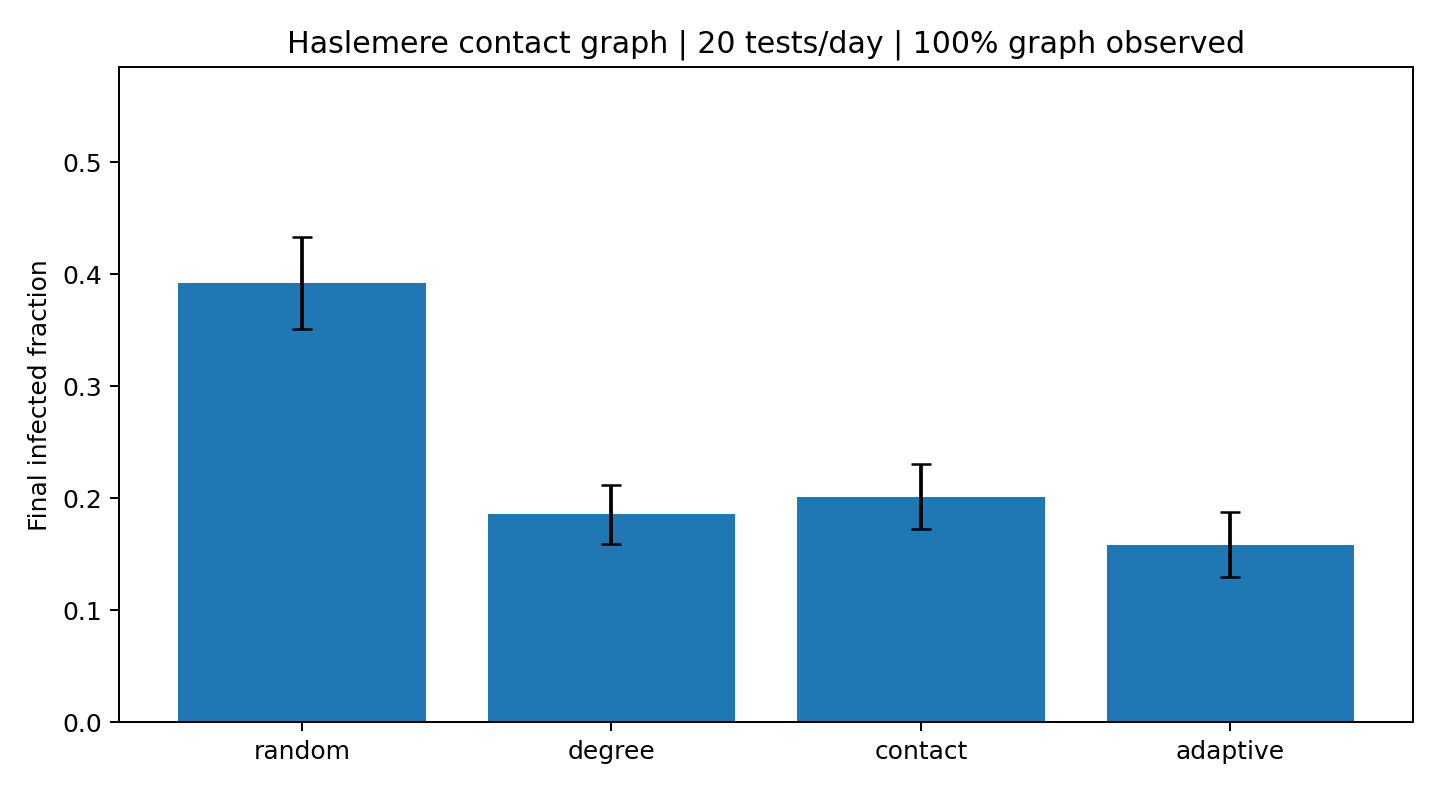
\includegraphics[width=0.56\linewidth]{figures/haslemere_policy.png}
\caption{Testing policies evaluated on the observed Haslemere contact topology. Error bars show 1.96 Monte Carlo standard errors.}
\end{figure}
